%%%%%%%%%%%%%%%%%%%%%%%%%%%%%%%%%%%%%%%%%%%%%%%%%%%%%%%%%%%%%%%%%%%%%%%%%%%%%%%%%%%%%%
% Figure 1
%%%%%%%%%%%%%%%%%%%%%%%%%%%%%%%%%%%%%%%%%%%%%%%%%%%%%%%%%%%%%%%%%%%%%%%%%%%%%%%%
\begin{figure}[H]
  \centering
  \resizebox {1.0\columnwidth} {!} {
    \begin{tikzpicture}[->,>=stealth',shorten >=1pt,auto,node distance=6cm, semithick]   
    \tikzstyle{every state}=[]
    \node[state] (A) [rectangle] {
      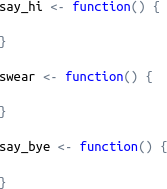
\includegraphics[width=0.2\textwidth]{1.png}
    };   
    \node[state] (B) [above right of = A, rectangle] {
      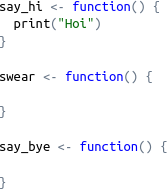
\includegraphics[width=0.2\textwidth]{2.png}
    };   
    \node[state] (C) [below right of = B, rectangle] {
      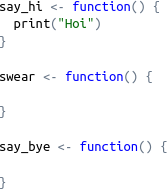
\includegraphics[width=0.2\textwidth]{2.png}
    };   
    \node[state] (D) [below right of = C, rectangle] {
      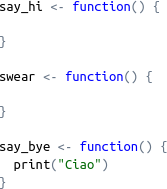
\includegraphics[width=0.2\textwidth]{3.png}
    };   
    \node[state] (E) [above right of = D, rectangle] {
      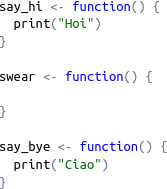
\includegraphics[width=0.2\textwidth]{4.png}
    };   
    \path 
      (A) edge [] node {} (B)
      (A) edge [] node {} (C)
      (B) edge [] node {} (C)
      (A) edge [] node {} (D)
      (C) edge [] node {} (E)
      (D) edge [] node {} (E)
    ; 
    \end{tikzpicture}
  }
\end{figure}
%%%%%%%%%%%%%%%%%%%%%%%%%%%%%%%%%%%%%%%%%%%%%%%%%%%%%%%%%%%%%%%%%%%%%%%%%%%%%%%%

%\newpage

%%%%%%%%%%%%%%%%%%%%%%%%%%%%%%%%%%%%%%%%%%%%%%%%%%%%%%%%%%%%%%%%%%%%%%%%%%%%%%%%%%%%%%
% Figure 1
%%%%%%%%%%%%%%%%%%%%%%%%%%%%%%%%%%%%%%%%%%%%%%%%%%%%%%%%%%%%%%%%%%%%%%%%%%%%%%%%
\begin{figure}[H]
  \centering
  \resizebox {1.0\columnwidth} {!} {
    \begin{tikzpicture}[->,>=stealth',shorten >=1pt,auto,node distance=6cm, semithick]   
    \tikzstyle{every state}=[]
    \node[state] (A) [rectangle] {
      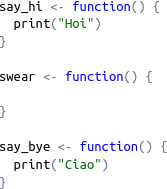
\includegraphics[width=0.15\textwidth]{4.png}
    };   
    \node[state] (B) [above right of = A, rectangle] {
      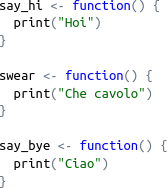
\includegraphics[width=0.15\textwidth]{5.png}
    };   
    \node[state] (C) [below right of = B, rectangle] {
      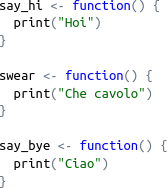
\includegraphics[width=0.15\textwidth]{5.png}
    };   
    \node[state] (D) [below right of = C, rectangle] {
      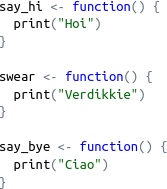
\includegraphics[width=0.15\textwidth]{6.png}
    };   
    \node[state] (E) [above right of = D, rectangle] {
      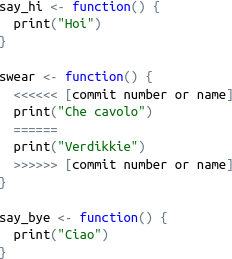
\includegraphics[width=0.15\textwidth]{7.png}
    };   
    \node[state] (F) [right of = E, rectangle] {
      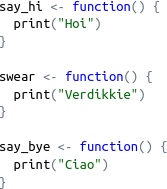
\includegraphics[width=0.15\textwidth]{8.png}
    };   
    \path 
      (A) edge [] node {} (B)
      (A) edge [] node {} (C)
      (B) edge [] node {} (C)
      (A) edge [] node {} (D)
      (C) edge [] node {} (E)
      (D) edge [] node {} (E)
      (E) edge [] node {} (F)
    ; 
    \end{tikzpicture}
  }
\end{figure}
%%%%%%%%%%%%%%%%%%%%%%%%%%%%%%%%%%%%%%%%%%%%%%%%%%%%%%%%%%%%%%%%%%%%%%%%%%%%%%%%

